\documentclass{scrreprt}
\usepackage[utf8]{inputenc}

\title{E-Learning und digitale Vorlesungsaufzeichnung}
\author{Denis Vogel, Johannes Alvarez}
\date{\today}


\usepackage[ngerman]{babel}
\usepackage[T1]{fontenc}
\usepackage{microtype}

\usepackage{natbib}
\usepackage{graphicx}
\graphicspath{ {images/} }

\usepackage{setspace}
\onehalfspacing

\begin{document}
\tolerance=500


\renewcommand\contentsname{Themen}


\maketitle
\tableofcontents


\chapter*{Über das Projekt}
Das folgende Dokument soll einen Überblick verschaffen über die Vorlesungsaufzeichnungsmethode der E-Learning Plattform MaMpf, über die diesbezüglichen technischen Anforderungen, den Nachbearbeitungsprozess via Schnittsoftware sowie weitere Möglichkeiten der digitalen Lerninhaltsvermittlung.
Hiermit soll aufgezeigt werden, dass mit einer vergleichsweise geringen Einarbeitungszeit und ohne großes technisches Fachverständnis ein verhältnismäßig intensiver Effekt auf und Mehrwert für die Lernstruktur der erreichten Studenten entstehen kann.\\
Aufgrund der simplen und verlässlichen Prozedur der Aufzeichnung und der etwaigen Möglichkeit, die Nacharbeit (d.h. den Schnitt, die Kapitelmarkierung, das Herausrechnen) durch studentische Hilfskraft erfolgen zu lassen, ist der Aufwand im Vergleich zum dadurch entstehenden immensen Nutzen für die Studenten verschwindend gering. Diese Anleitung/Übersicht wird nun im Folgenden zuerst einen kurzen technischen Überblick geben und in detailierter Weise auf die Grundlagen und den Ablauf der Aufzeichnung eingehen, anschließend eine genaue „Schritt-für-Schritt“-Anleitung zum Nachbearbeitungsprozess bereitsstellen und zu guter Letzt in Verbindung zu weiteren Angeboten der Plattform MaMpf auf zusätzliche Vorteile der modernen digitalen Vermittlung von Lerninhalten eingehen. 


\chapter{Das technische Fundament}

\section{Die Hardware-Voraussetzungen}

Bei der Aufzeichnungsmethode KaViaR (Kameraloses Videoaufzeichnungssystem zur Rekapitulationsunterstützung) handelt es sich -- wie der vollständig ausgeschriebene Name bereits sagt -- um ein Aufnahmeverfahren, dass vollständig digital erfolgt und keine Kamera benötigt. Hierbei wird das klassische Tafelbild mit Kreideaufschrieb durch den Einsatz eines stiftfähigen Tablets mit entsprechender Notizsoftware ersetzt. Das Bildschirmsignal des Tablets wird während der Vorlesung per Beamer an eine Leinwand projiziert und parallel aufgezeichnet (weiteres dazu im nächsten Unterkapitel). In einem ersten Versuch im WS 16/17 wurde dafür ein Microsoft Surface Book verwendet. Für eine optimale Aufnahme des Audioinhaltes wird zudem ein externes Mikrofon mit Nierencharakteristik und Phantomspeisung benötigt, welches durch mehrere Adapter am Laptop angeschlossen wird.
\\Um die aufgezeichnete Vorlesung anschließend mit Camtasia nachbearbeiten zu können, wird ein verhältnismäßig leistungsstarker Rechner benötigt, welcher sowohl die benötigte Zeit des „Renderns“ (Herausrechnen des Videos), als auch die der Transkodierung (Umwandlung und Komprimierung eines Dateiformats) stark verkürzt.

\bigskip
\bigskip
\textbf{Eine technische Übersicht der verwendeten Hardware:}

\begin{itemize}
  \item Microsoft Surface Book mit Core i7-Prozessor, 16 GB RAM und 1 TB SSD
  \item Mini-XLR-Headset-Mikrofon (Omnitronic HS-1100)
  \item Adapter Mini-XLR  $\rightarrow$ XLR mit Phantomspeisung (StageLine EMA-300P)
  \item Adapter XLR  $\rightarrow$ USB (Shure X2U)
  \item PC zur Video-Nachbearbeitung (mit Core i7-6700K-Prozessor, 32GB RAM, 1 TB SSD, 4TB HDD, NVidia Geforce 1070GTX Grafikkarte)
\end{itemize}

\section{Aufzeichnung mit Camtasia}
Ist die Hardware vollständig eingerichtet, kann mit Camtasia die Aufzeichnung des Bildschirmsignals gestartet werden. Es ist kein separates Aufnahmeprogramm für das Audiosignal erforderlich, da Camtasia dazu in der Lage ist, das externe Mikrofon abzugreifen. Sind der richtige Bildausschnitt sowie das externe Mikrofon ausgewählt, kann die Aufnahme durch Drücken auf den großen roten ''rec''-Knopf gestartet werden.
\\
\begin{figure}[h]
    \centering
    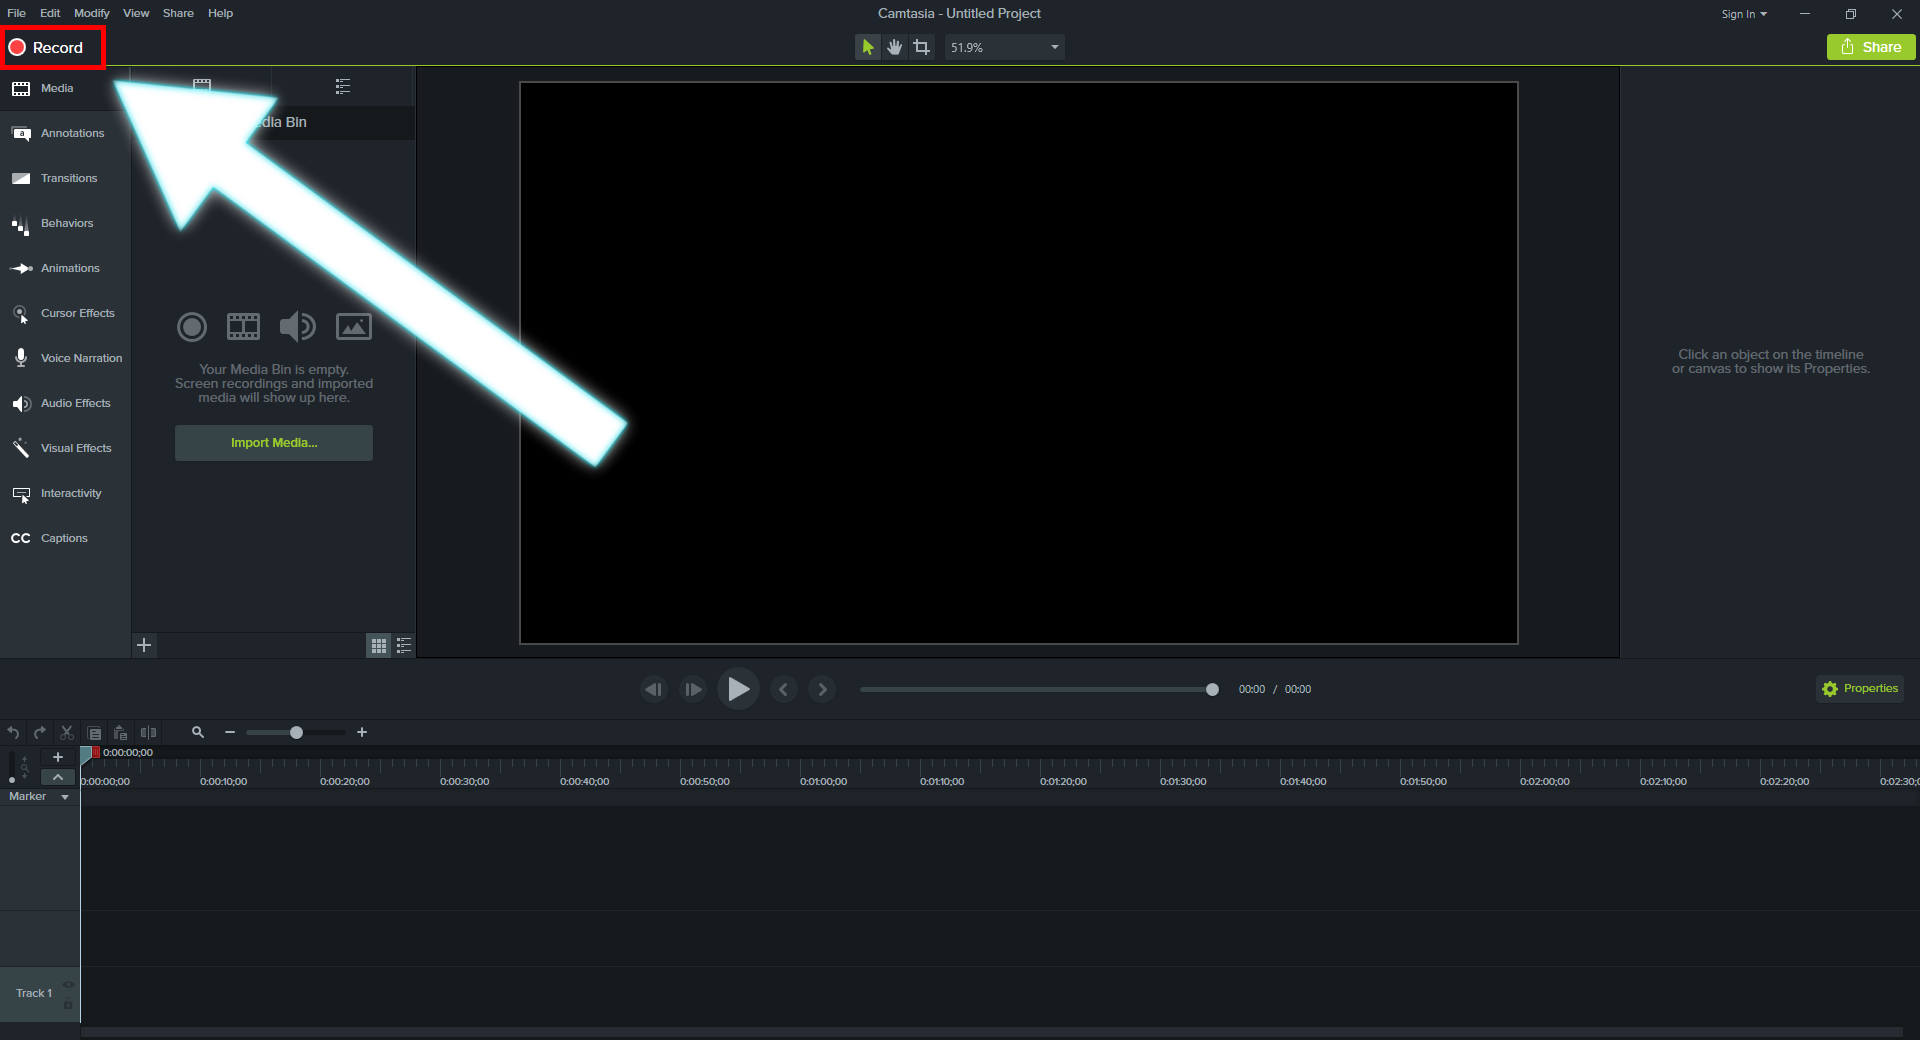
\includegraphics[width=1\textwidth]{record.png}
    \caption{Der Aufnahmeknopf befindet sich im linken oberen Bildschirmrand}
    \label{fig:record}
\end{figure}
\\
Der Unterrichtende hält nun unter Verwendung des Tablets und des Notizprogrammes die entsprechende Vorlesung. Nach Beendigung der Unterrichtseinheit drückt der Unterrichtende schließlich die ''F10''-Taste um die Aufnahme zu stoppen. Im ''Media bin'' oberhalb des Zeitstrahls sollte nun die entstandene ''.trec''-Datei der Vorlesungsaufzeichnung angezeigt werden. Durch einen Rechtsklick auf die Datei $\rightarrow$ ''Open file location'' kann nun der Speicheort dieser eingesehen werden. Von diesem Punkt an kann schließlich die Nacharbeitung beginnen.
\pagebreak
\begin{figure}[h]
    \centering
    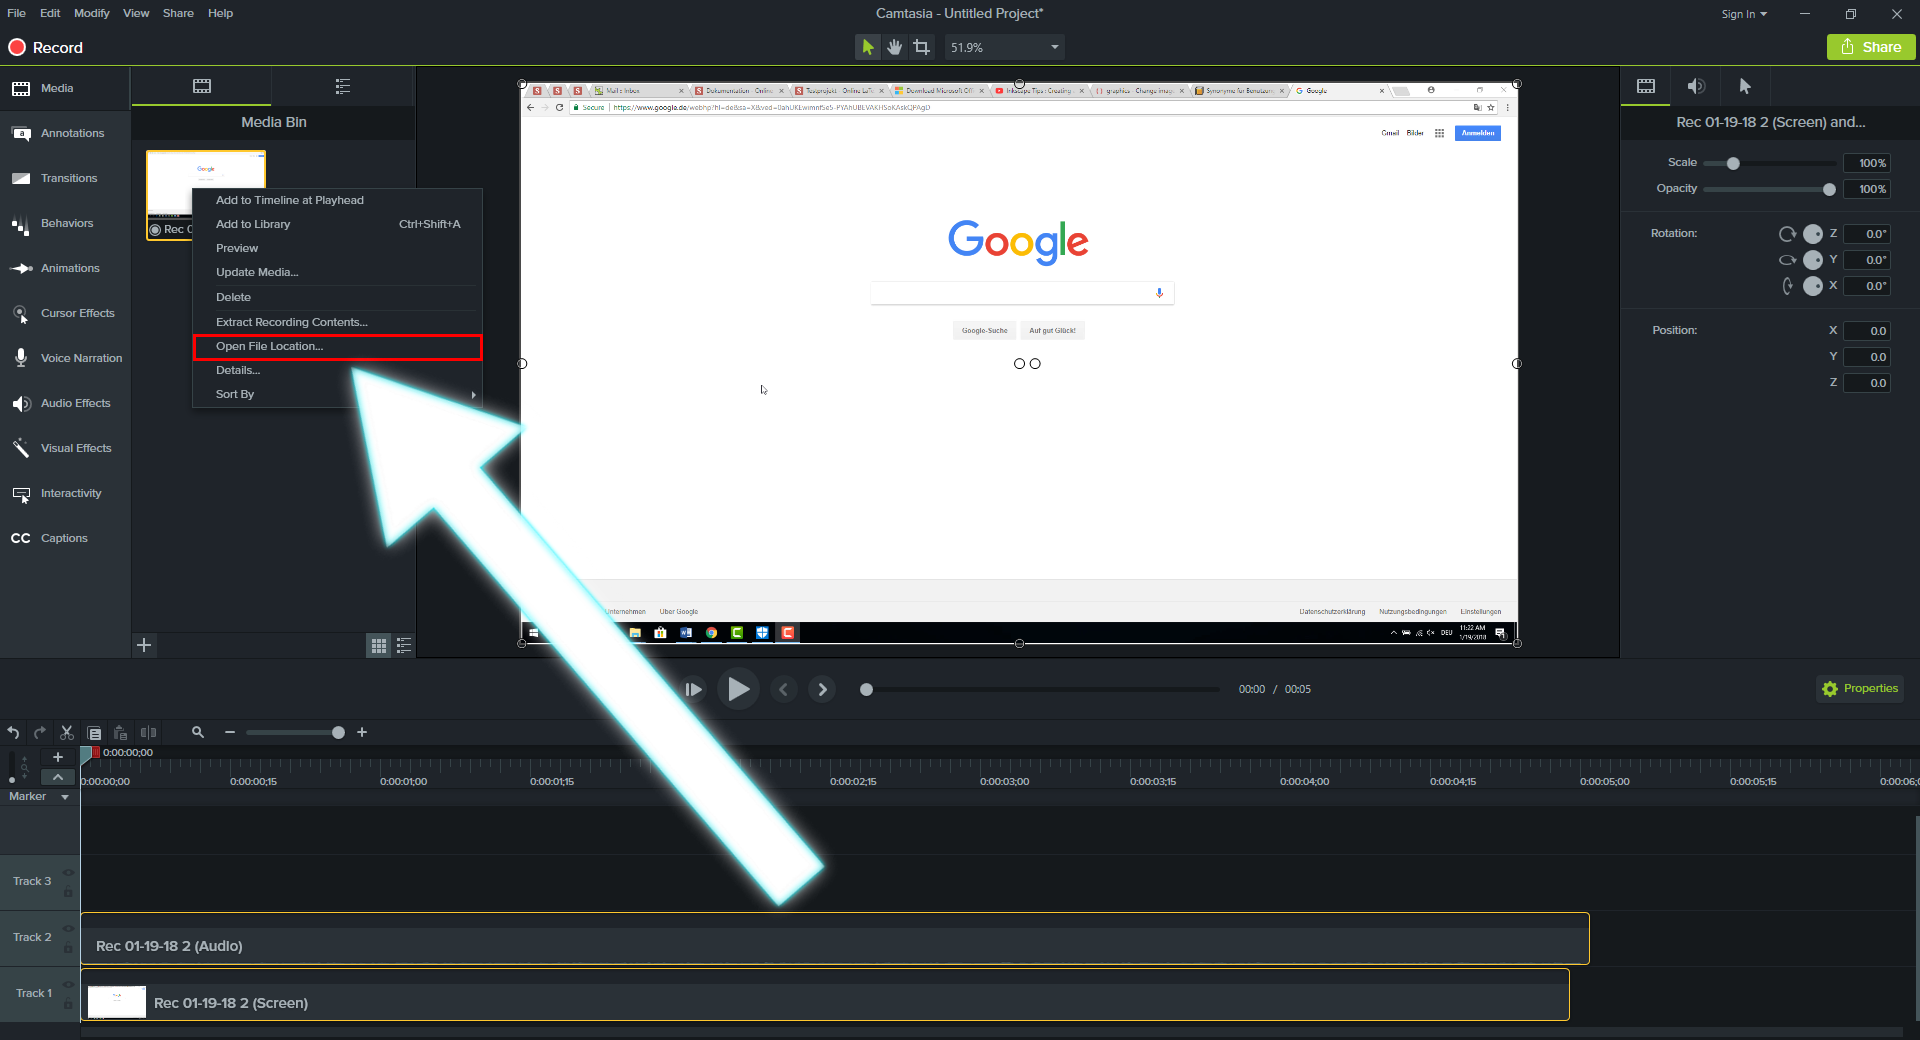
\includegraphics[width=1\textwidth]{filelocation}
    \caption{Auf diese Weise lässt sich das entstandene File finden}
    \label{fig:filelocation}
\end{figure}
\section{Zusätzliche Software}
Zusätzlich zur bereits erwähnten Videobearbeitungs- und Aufnahmesoftware Camtasia wird zur Transkodierung, also zur Dateikomprimierung und -umwandlung, das Programm MediaCoder benötigt. Der Vorlesungsaufschrieb wiederum wird mit dem Programm Microsoft OneNote erstellt. Für den seltenen Fall, dass die Audiospur ebenfalls Nacharbeitung benötigt, kann beispielsweise das kostenfreie Programm Audacity benutzt werden. 
\newpage 
\chapter{Nachbearbeitung des Videomaterials}
\section{Separierung von Audio und Video, Transkodierung}
Im ersten Schritt der Nachbearbeitung muss aus der durch die Aufnahme entstandenen .trec-Datei jeweils die entsprechende Video- (.avi) und Audiospur (.wav) extrahiert werden. Klicken Sie dafür per Rechtsklick auf die Datei im ''Media bin'' und anschließend auf ''Extract recording contents''. Dieser Vorgang muss zwei mal durchgeführt werden, wobei einmal der Haken ''Screen Video'' und einmal der Haken ''Microphone Audio'' gesetzt sein muss. 
\begin{figure}[h]
    \centering
    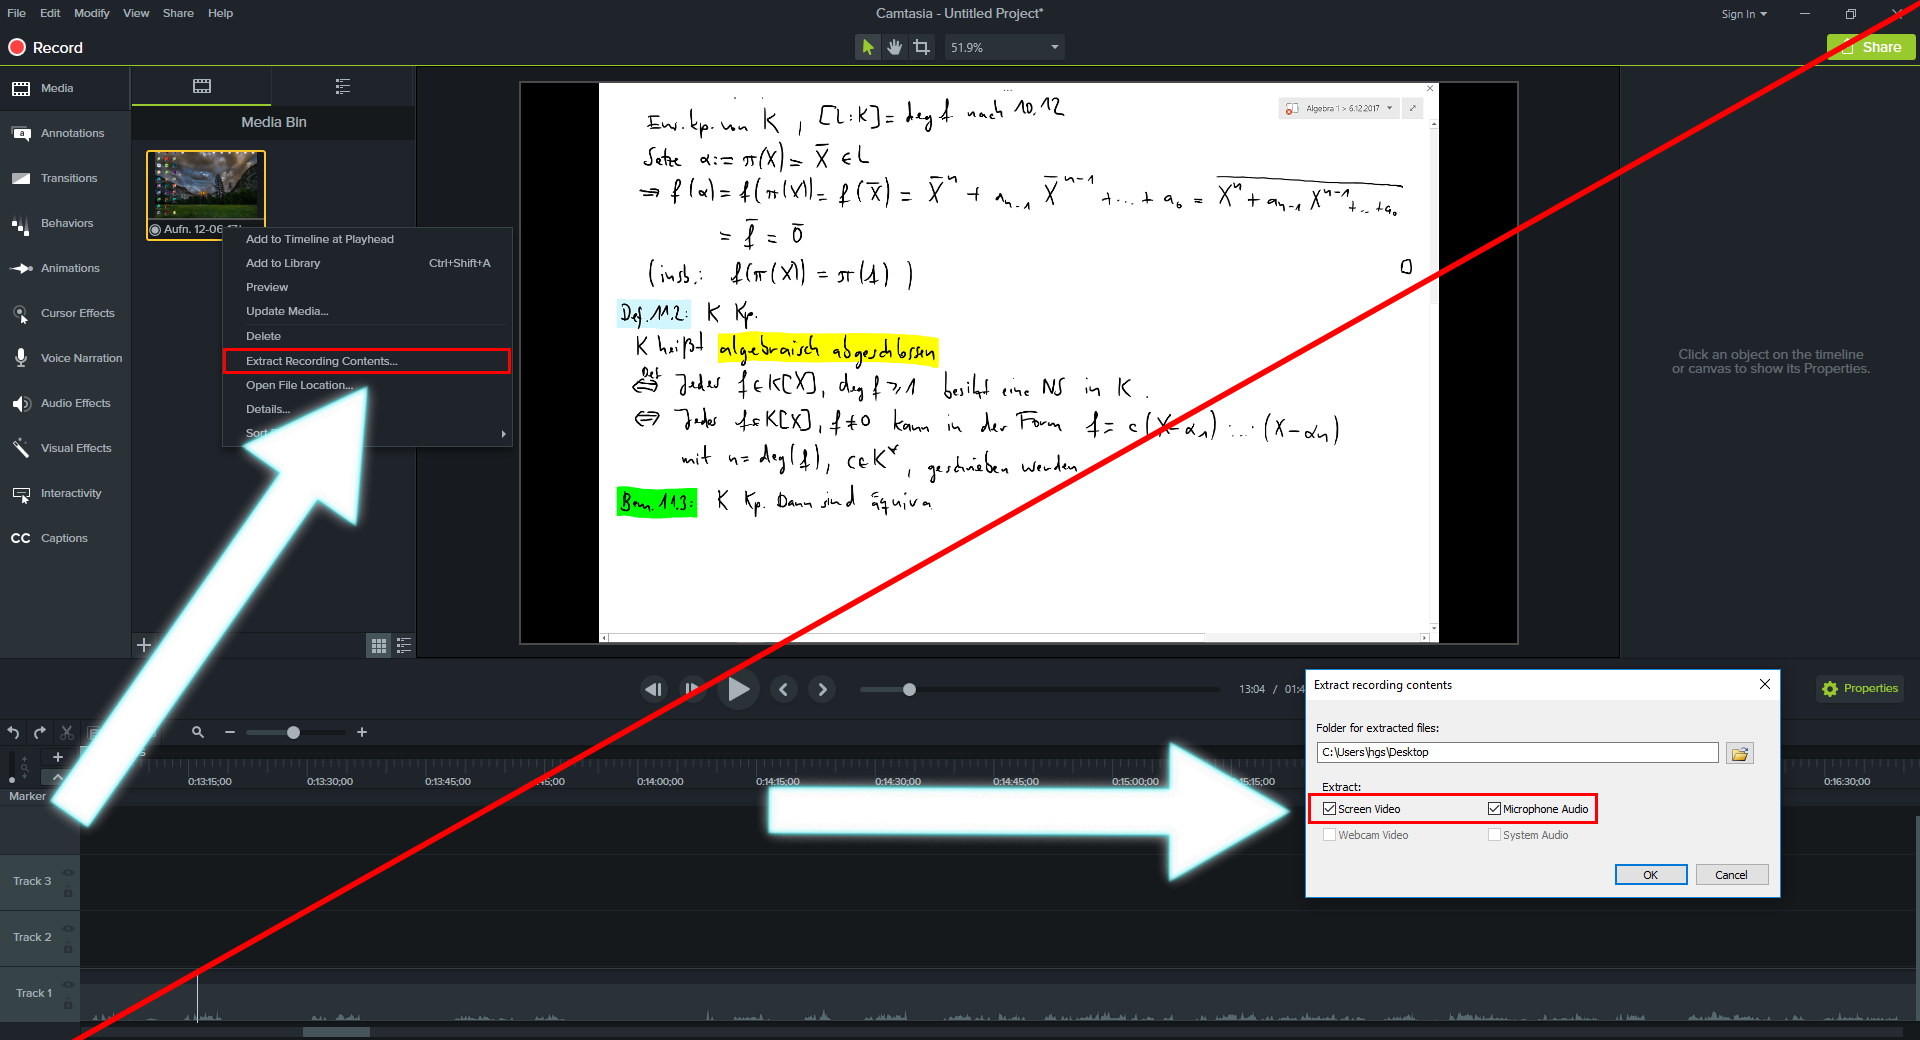
\includegraphics[width=1\textwidth]{extractrecordingcontents.png}
    \caption{Aus der entstandenen .trec-Datei müssen zuallererst Video und Audio extrahiert werden}
    \label{fig:extractrecordingcontents}
\end{figure}
\\ 
Die dabei entstehende Audiodatei kann im Normalfall unverändert weiterverwendet werden. Die Videodatei hingegen muss nun mit dem MediaCoder bearbeitet werden. Die nötigen Voreinstellungen für die ideal komprimierte Datei finden sich in einem beigefügten XML. Über ''File'' $\rightarrow$ ''Load Preset'' kann dieses in MediaCoder verwendet werden.
\\
\begin{figure}[h]
    \centering
    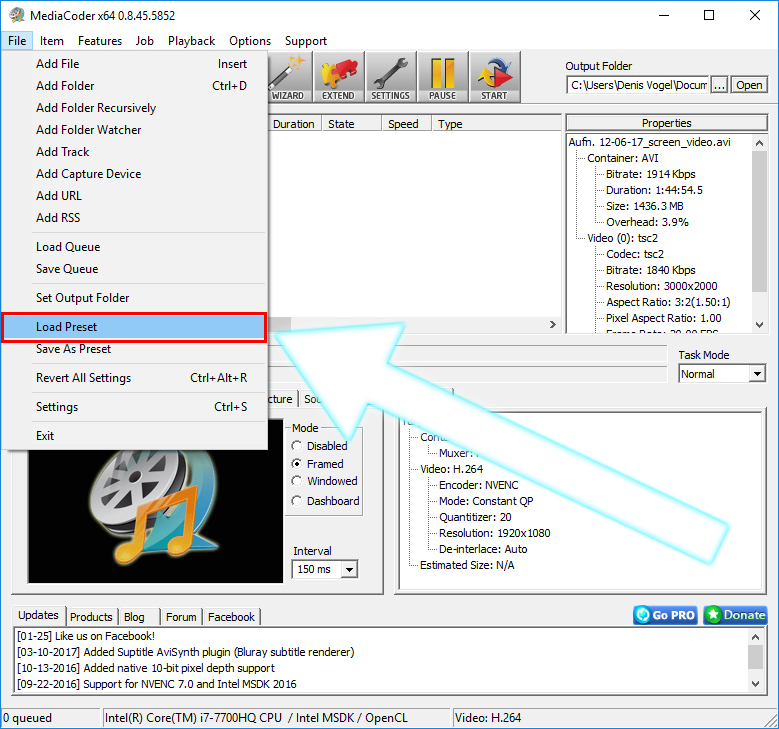
\includegraphics[width=1\textwidth]{mediacoder.png}
    \caption{Die optimierten Einstellungen für den MediaCoder lassen sich mit dem XML-File einfach übertragen, was weitere Anpassungen obsolet macht}
    \label{fig:mediacoder}
\end{figure}
\\
Klicken Sie auf ''Start'' um die Transkodierung zu starten. Die hierbei entstehende .mp4-Datei sowie die zuvor extrahierte .wav-Datei können nun mit Camtasia weiter bearbeitet werden.
\\
\pagebreak
\section{Schnittarbeit mit Camtasia}
Die Video- und Audiodatei sowie das der Vorlesung entsprechende Intro-Video müssen nun in Camtasia durch ''Import Media'' oder den Zugriff auf die Library (siehe Bild) in das Projekt importiert werden. Im nächsten Schritt wird zunächst die Audiodatei auf ''Track 1'' gesetzt und anschließend die Videodatei auf ''Track 2''. Dabei muss darauf geachtet werden, dass beide Spuren zum Zeitpunkt 0 (siehe Zeitstrahl oberhalb) beginnen, also synchron zueinander sind.
\\Um zu vermeiden, dass im weiteren Schnittprozess nicht versehentliche eine Asynchronität entsteht, indem nur das Videoelement oder nur das Audioelement verschoben wird, können beide Einheiten selektiert und Gruppiert werden (''STRG + G'' oder Rechtsklick $\rightarrow$ ''Group''). Auf eine dritte Spur (''Track 3'') wird nun mit leichter Überblendung zum Vorlesungsvideo das Intro gezogen. Bei Bedarf kann hier noch ein überblendender Effekt eingefügt werden (''Transistions'' $\rightarrow$ ''Fade'' $\rightarrow$ auf das Ende der Introspur ziehen).
\\
\begin{figure}[h]
    \centering
    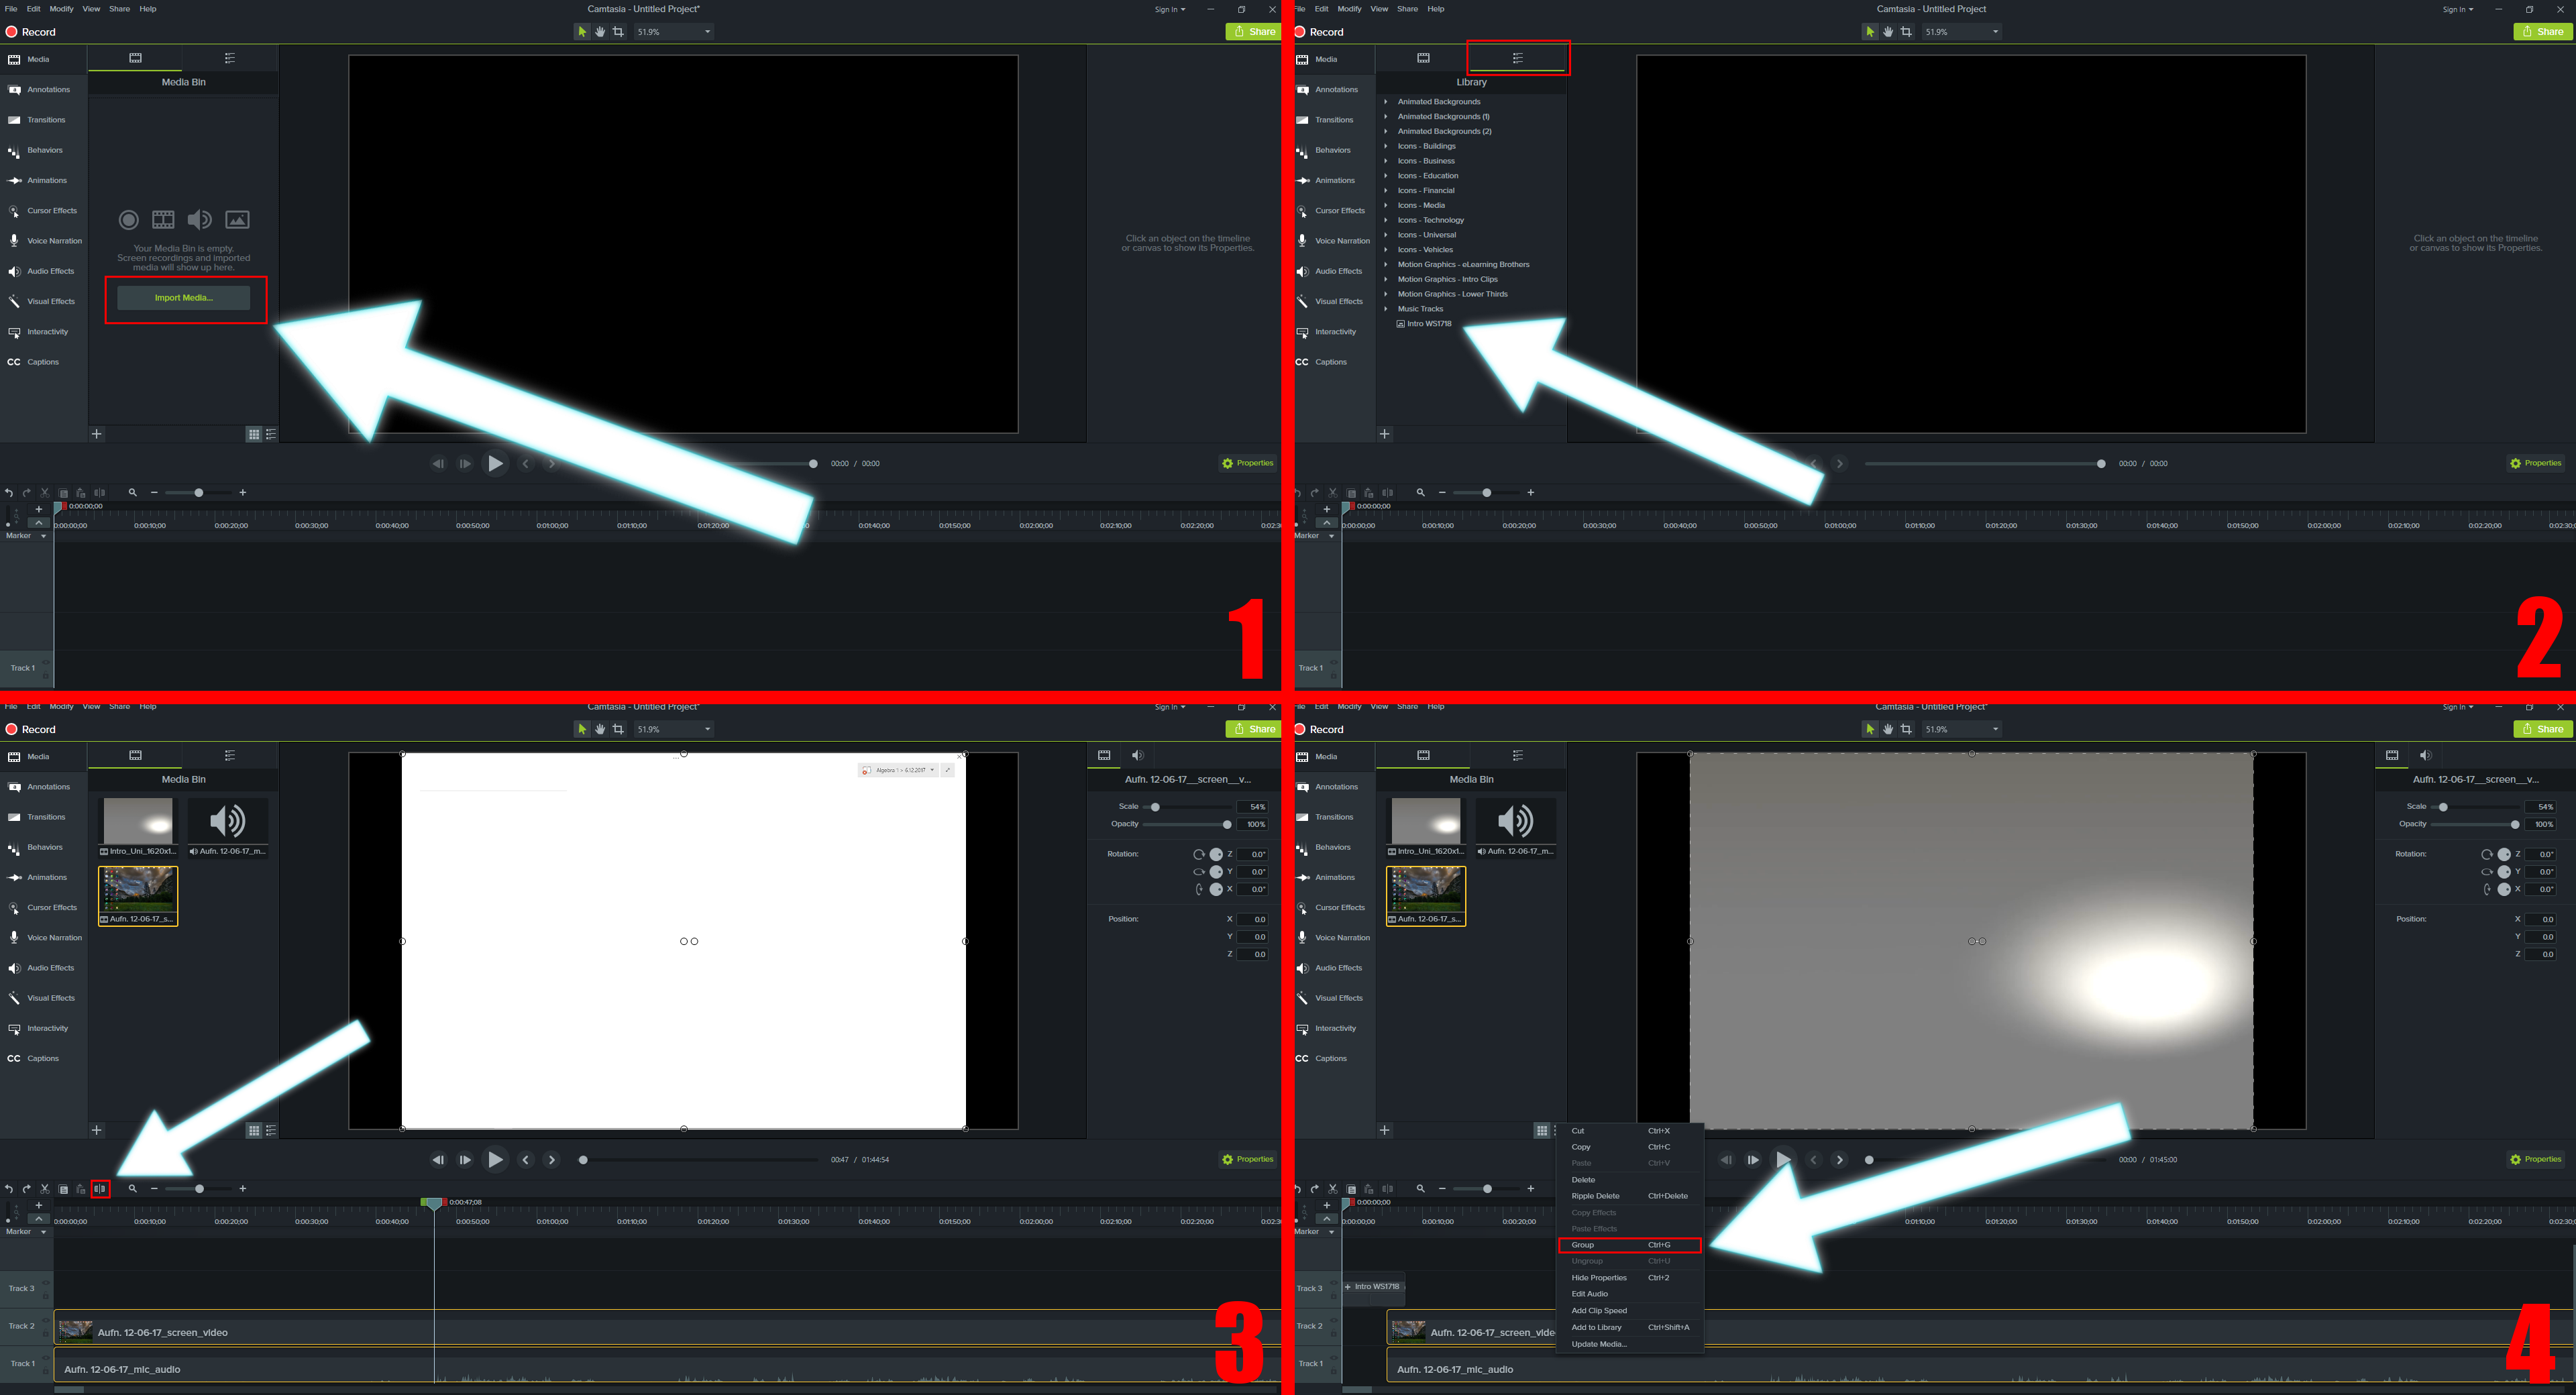
\includegraphics[width=1\textwidth]{foursteps.png}
    \caption{Importieren, Gruppieren, Wegschneiden des Anfangs und Einfügen des Intros}
    \label{fig:foursteps}
\end{figure}
\pagebreak
\\
Nun kann durch Verschieben des Cursors oder via Klicken auf die jeweiligen Stellen im Zeitstrahl zunächst an die Stelle gesprungen werden, an der die Vorlesung, also das Video, inhaltlich beginnt. Ist eine geeignete Stelle gefunden, an der das Video später starten soll, muss das gruppierte Elemente des Vorlesungsvideos ausgewählt und mit ''S'' (Split) oder durch Drücken des entsprechenden Symbol ein Schnitt gesetzt werden. Der dadurch entstandene überflüssige Anfang des Videos kann nun markiert und gelöscht werden.\\
Zusätzlich zum Anfang muss zudem noch der ''leere'' Mittelteil (5-Minuten-Pause) und das Ende passend weggeschnitten werden. Dafür wird der bereits beschriebene Vorgang wiederholt (Entsprechende Stellen durch Verschieben des Cursors heraussuchen, die notwendigen Schnitte mit ''S'' setzen, die zu entfernenden Spurelemente markieren, herauslöschen und beim Schnitt im Mittelteil die Spuren wieder nahtlos zusammenschieben).\\
Ist dieser Punkt erreicht, sind also Anfang, Mittelteil und Schluss zurechtgeschnitten und ist das Intro hinzugefügt, kann mit dem inhaltlichen Markieren der einzelnen Vorlesungselemente begonnen werden. Camtasia bietet die Möglichkeit, mit diesen Markierungen eine Inhaltsangabe für Videos zu erstellen. 
\\
\begin{figure}[h]
    \centering
    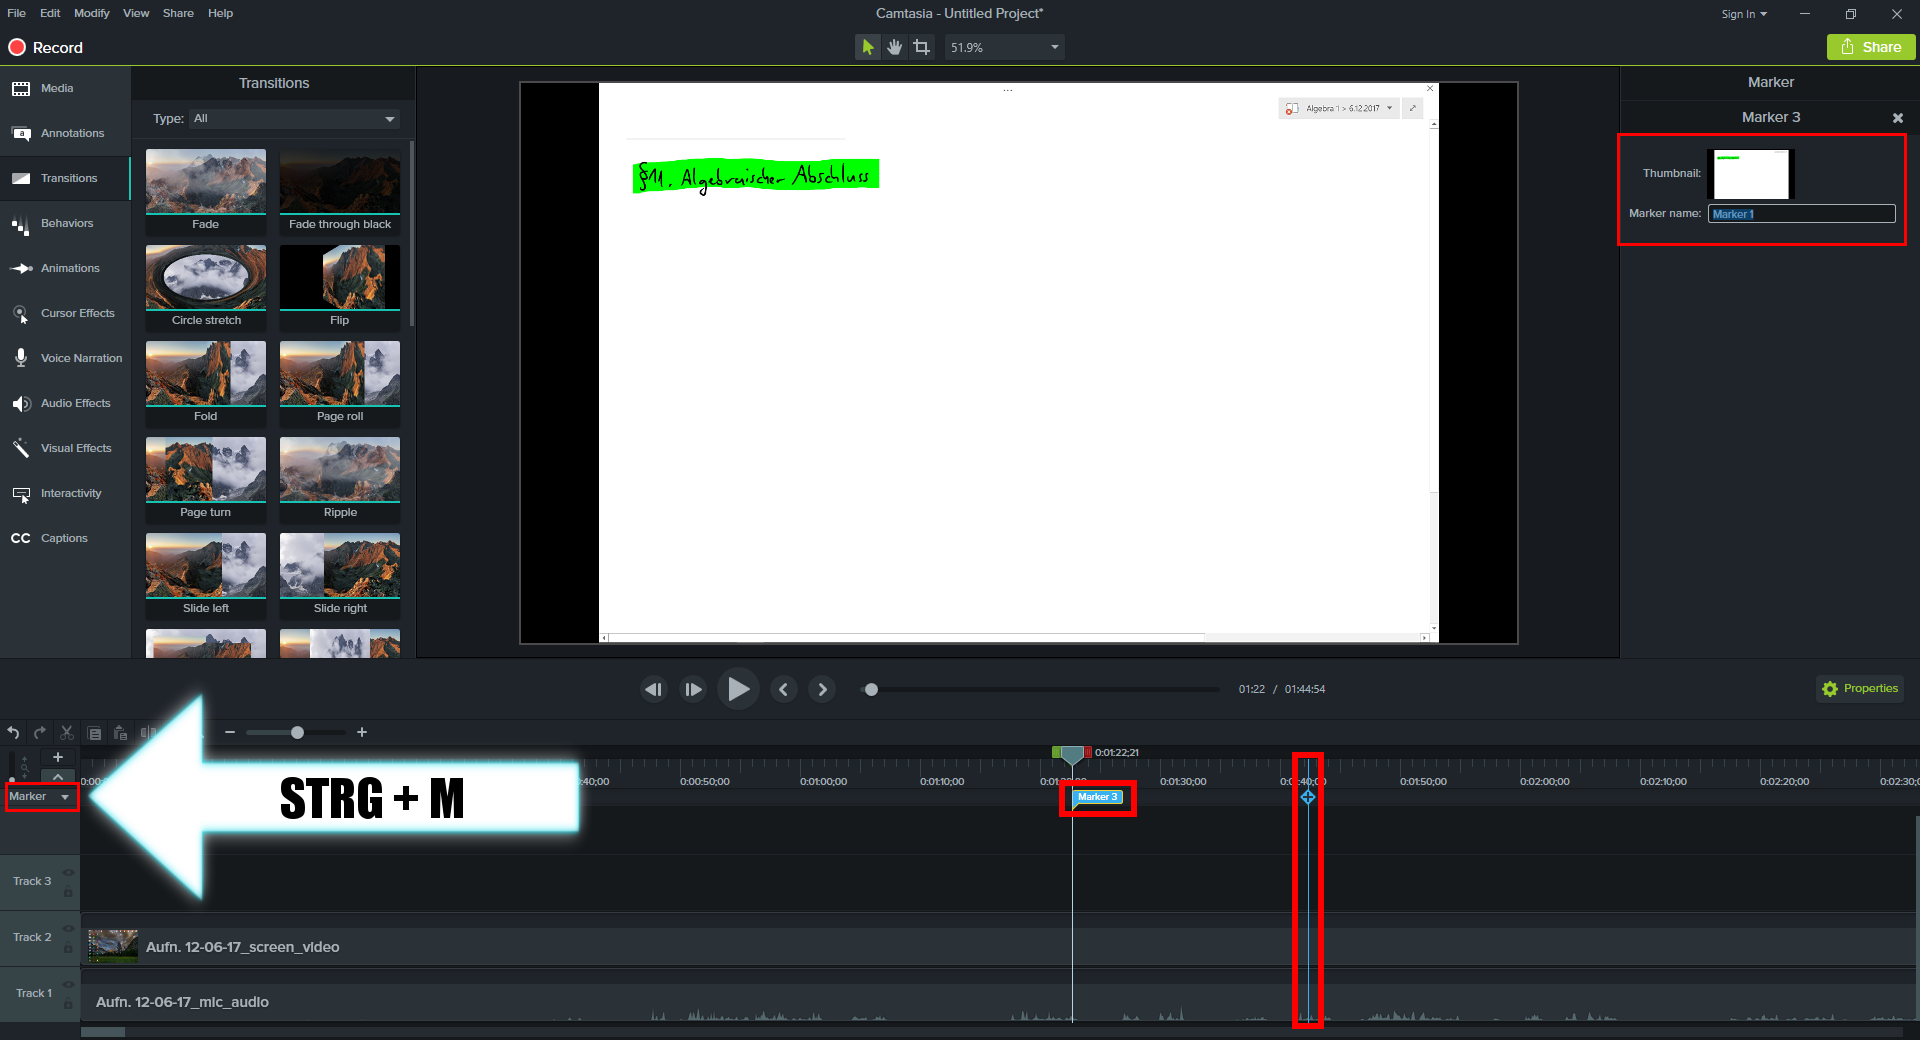
\includegraphics[width=1\textwidth]{markierungen.png}
    \caption{Die Markierungsfunktion bietet die Möglichkeit, eine Inhaltsangabe für das Video zu erstellen}
    \label{fig:markierungen}
\end{figure}
\pagebreak
\noindent
\\
Die Funktion lässt sich mit ''STRG + M'' ein- und ausschalten. Die Marker können per Mausklick auf die entsprechende Stelle innerhalt des Zeitstrahls, oder per ''SHIFT + M'' an die momentane Position des Cursers gesetzt werden. Im rechten oberen Bildschirmbereich kann der Marker anschließend noch, entsprechend des an der jeweiligen Stelle im Video behandelten Inhaltes, umbenannt werden. Die Inhaltsangabe ermöglicht es dem Betrachter, direkt an bestimmte Stellen des Videos zu springen, von daher ist es notwendig, die Vorlesung nochmals sorgsam von Anfang bis Ende durchzugehen und die entsprechenden Markierungen so zu benennen und zu platzieren, dass der Rezipient den größtmöglichen Vorteil von dieser Funktion hat. Sind alle Marker schließlich gesetzt, ist die Nachbearbeitung mit Camtasia abgeschlossen.

\section{Stopfunktion am Ende eines Videos, Link einbauen}
Eine für die Studenten nützliche Videofunktion, die Camtasia anbietet, ist die Möglichkeit, das entsprechende Video nach vollständigem Abspielen automatisch anzuhalten. Dies ist von daher gewinnbringend, da das Video im Normalfall wieder an den Anfang springen würde, und so Studenten, die parallel zur digitalen Vorlesung mitschreiben, den letzten Teil des Videos in Ruhe notieren können, ohne manuell wieder ans Ende springen oder das Video selbst anhalten zu müssen. Hierfür wird aus den verfügbaren ''Annotations'' eine weiße Box ausgewählt und diese -- einen Track über die Vorlesungsspur an deren Ende platziert. Auf der Timeline soll dieses Element nun an der Stelle beginnen, an der das Video angehalten werden soll. Gleichzeitig muss auf dem Vorschaubildschirm die entsprechende Anmerkung klein gezogen und in die Bildschirmecke positioniert werden.
\pagebreak\\
Im nächsten Schritt soll nun der Beispieltext der Anmerkung entfernt werden und in den Einstellungen die beiden ''Opacity''-Regler auf 0 gesetzt werden, womit die Anmerkung ihre Sichtbarkeit verliert. Anschließend soll nun unter ''Visual Effects'' $\rightarrow$ ''Interactive Hotspot'' der notwendige Effekt auf das Element der Anmerkung gezogen werden. Nun muss nur noch sichergestellt werden, dass der Haken bei ''Pause at End'' gesetzt ist.
\\
\begin{figure}[h]
    \centering
    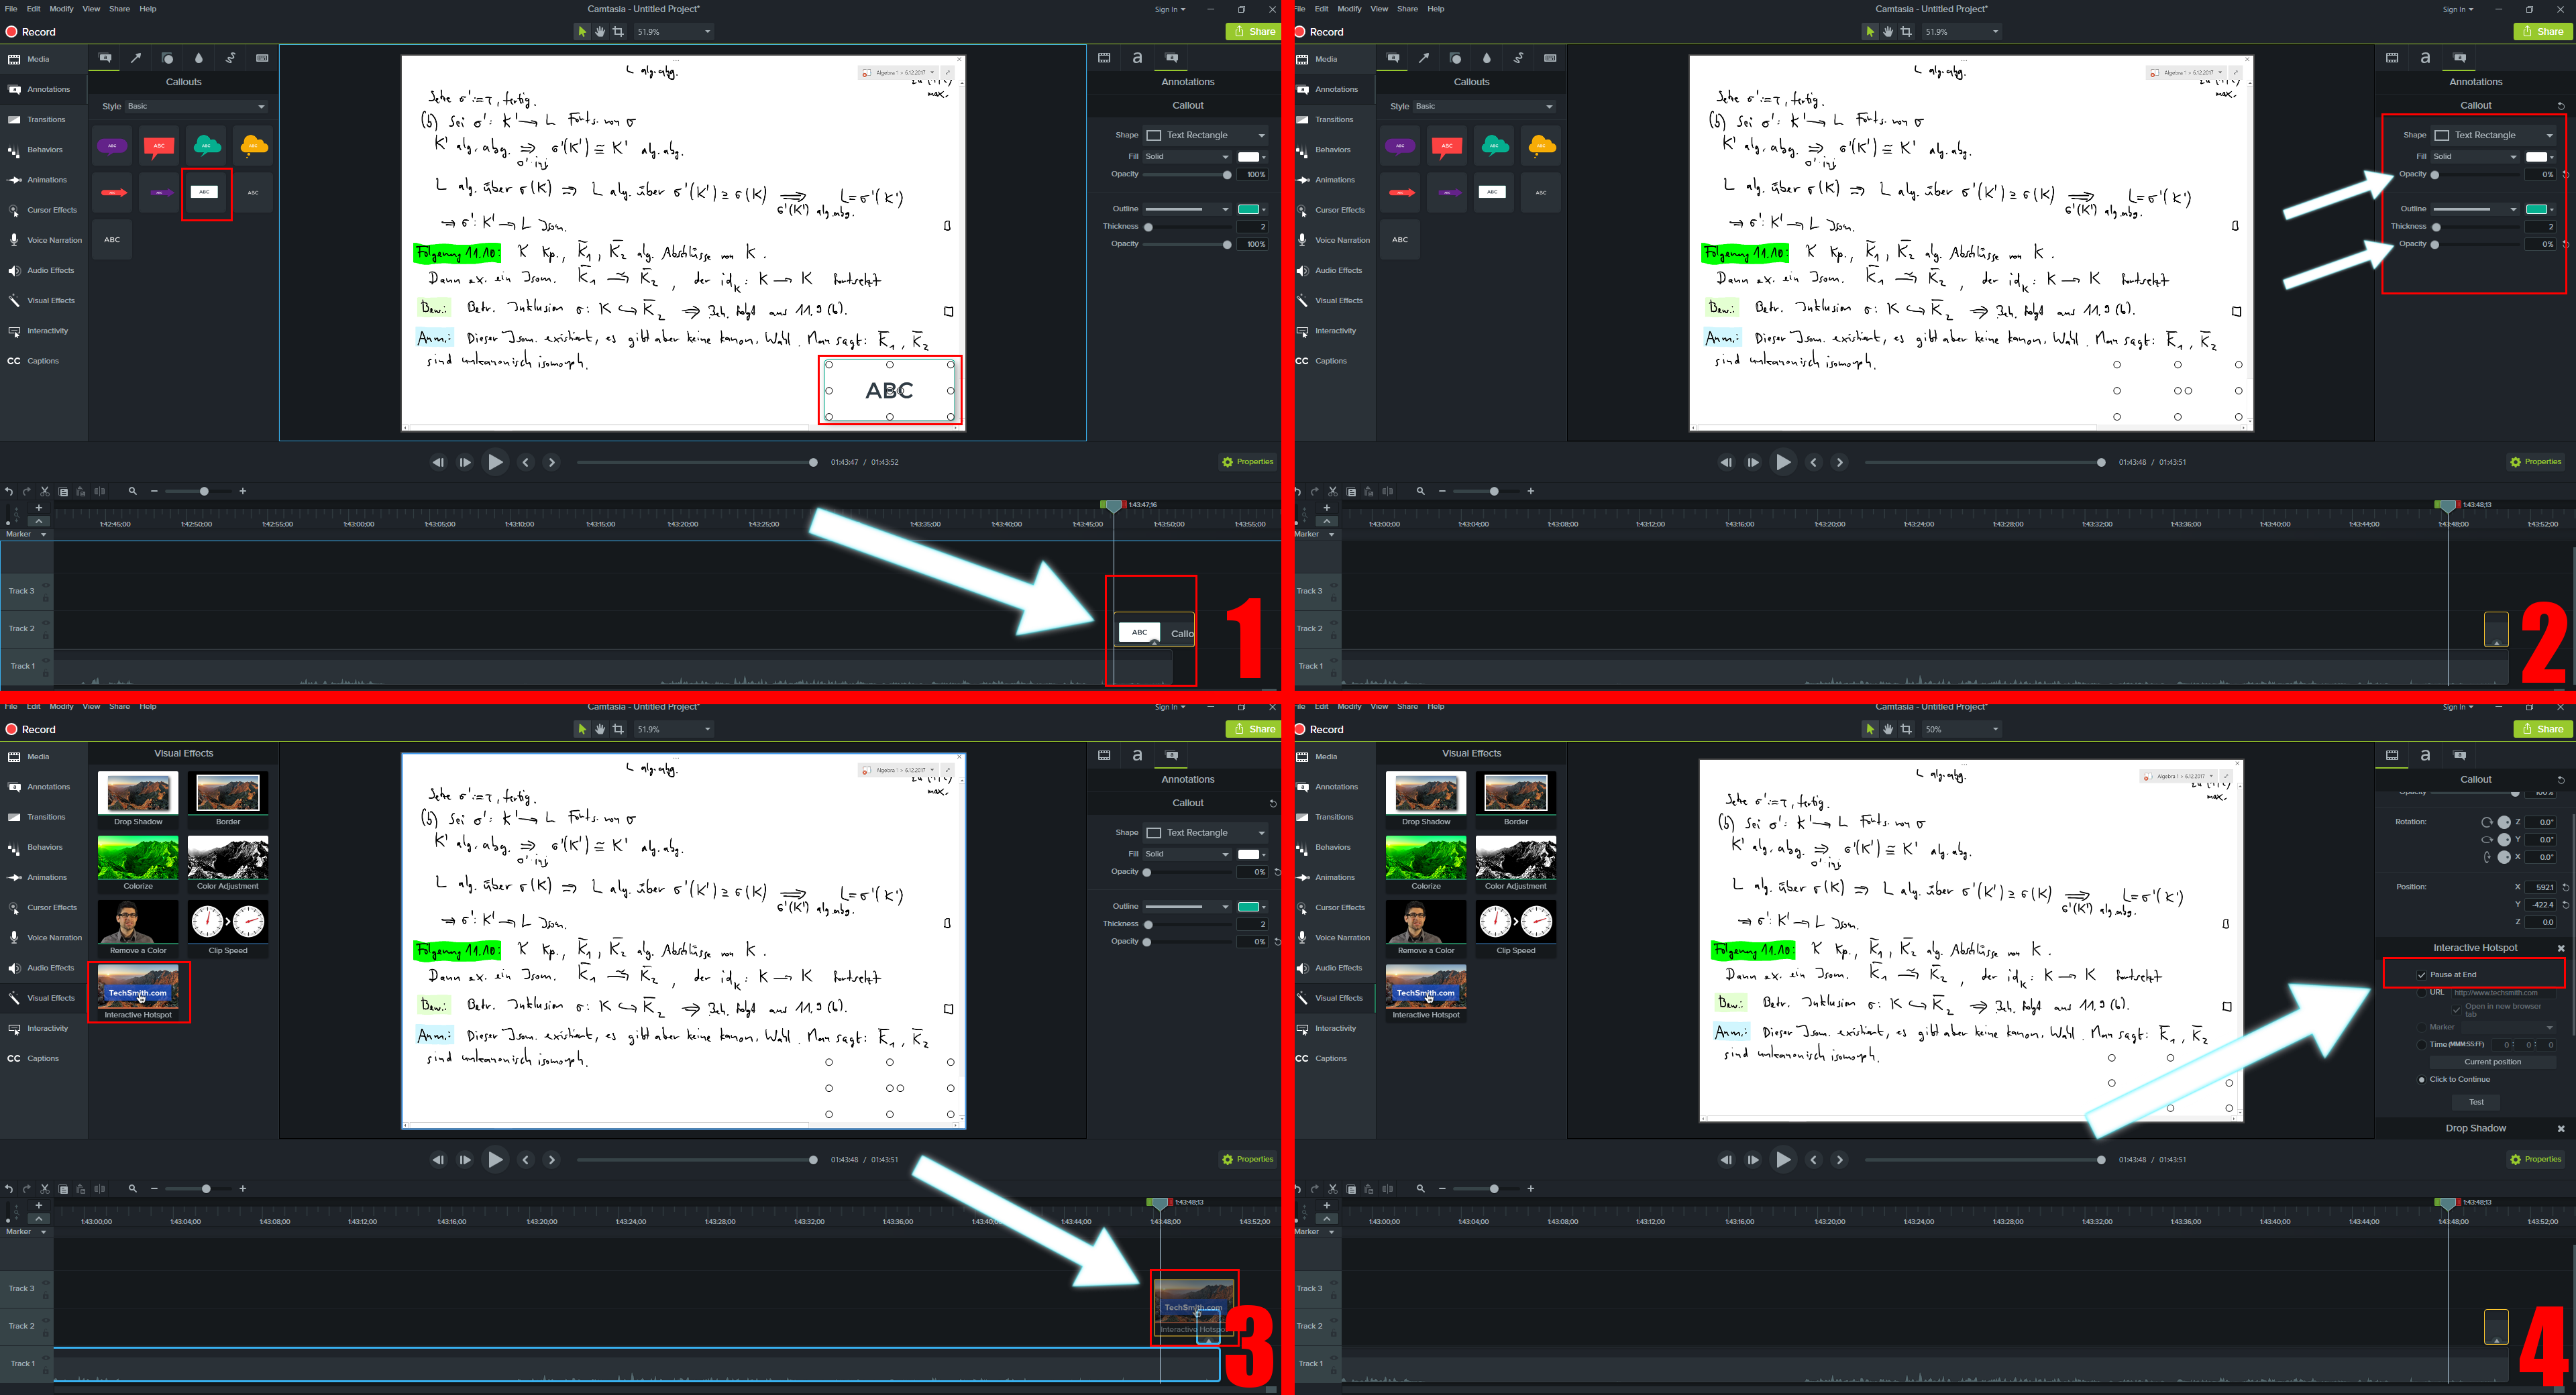
\includegraphics[width=1\textwidth]{endvideo.png}
    \caption{Über eine mit Anhaltfunktion versehene Annotation, die nicht sichtbar im Bildausschnitt platziert wird, wird verhindert, dass das Video, wenn es schließlich von Studenten angesehen wird, am Ende wieder ungewollt von vorne startet}
    \label{fig:endvideo}
\end{figure}
\\
In der beinahe gleichen Art lässt sich zudem auch innerhalb des Videos ein Link einfügen, welcher beispielsweise zu einem hochgeladenen PDF-Dokument mit detaillierteren Erklärungen führt. Dafür muss der Haken bei ''URL'' gesetzt (''Pause at End'' hier nicht notwendig) und in das Feld die entsprechende Adresse eingefügt werden. Bei einer solchen Anmerkung ist es sinnvoll, die Einstellungen zur ''Opacity'' unverändert zu lassen und den Link durch Änderung des Beispieltextes kurz zu beschreiben.
\pagebreak 
\section{Tipps und Tricks für den Videoschnitt}
Für manche Probleme die bezüglich des Videoschnitts  eintreten können, lassen sich keine standardisierten Anleitungen geben. Für diese muss der Editor des Videos eigene kreative Lösungsansätze finden. Ein Beispiel hierfür: Das Video beinhaltet eine falsche Information, eine falsche Benennung eines mathematischen Begriffes oder Ähnliches. In diesem Fall gibt es mehrere Lösungen. Eine davon wäre, eine bestimmte Szene neu aufzuzeichnen oder zu vertonen. Falls die falsch gegebene Information nur auf der Tonspur stattfindet und im Video bereits an anderer Stelle richtig gegeben wurde, ließe sich allerdings auch das richtige Ton-File herauskopieren und an der falschen Stelle einfügen. Hierbei muss allerdings darauf geachtet werden, dass sich das entsprechende kopierte Element organisch in die bestehende Tonspur einfügen lässt. 

Ein weiterer Aspekt betrifft den Umgang mit längeren Schreibszenen in denen auf der akkustischen Ebene. Um eine solche Spur, auf der auf der inhaltlichen Ebene Leere und ledigliche der Schreibprozess abgewartet werden muss, lässt sich die entsprechende Videospur beschleunigt darstellen, währenddess die Audiospur entweder entfernt oder ebenfalls verkürzt wird. Dies ist möglich per Rechtsklick auf die entsprechende Spur und ''Add Clip Speed''. Weitergehend sollte darauf geachtet werden, die Tonspur in einer Art und Weise zu editieren, sodass Störgeräusche auf ein Minimum beschränkt sind. Entsprechende Stellen können einfach aus der Spur heraus separiert und stummgeschaltet oder entfernt werden. Dies bedeutet jedoch nicht, dass jede Atempause entfernt werden muss: Ein natürlicher und angenehmer Sprachklang entsteht erst dadurch, gewisse Pausen im menschlichen Sprachfluss unbearbeitet zu lassen, da eine allzu robotisch und abgehackt klingende Tonspur auch negativ aufgenommen werden kann.




\pagebreak
\section{Fertigstellung und Einspeisung in die E-Learning Plattform}
Das fertig nachbearbeitete Video muss nun noch rausgerechnet werden. Dafür muss zunächst die Auflösung in den Projekteinstellungen angepasst werden. Mit Rechtsklick auf den Vorschaubildschirm $\rightarrow$ ''Project settings'' kann diese editiert werden. Die vorgegebenen Angaben nun durch die Auflösung ''1620x1080'' austauschen und abspeichern. Im nächsten Schritt auf ''Share'' $\rightarrow$ ''Local file'' im rechten oberen Bildschirmrand klicken.
\begin{figure}[h]
    \centering
    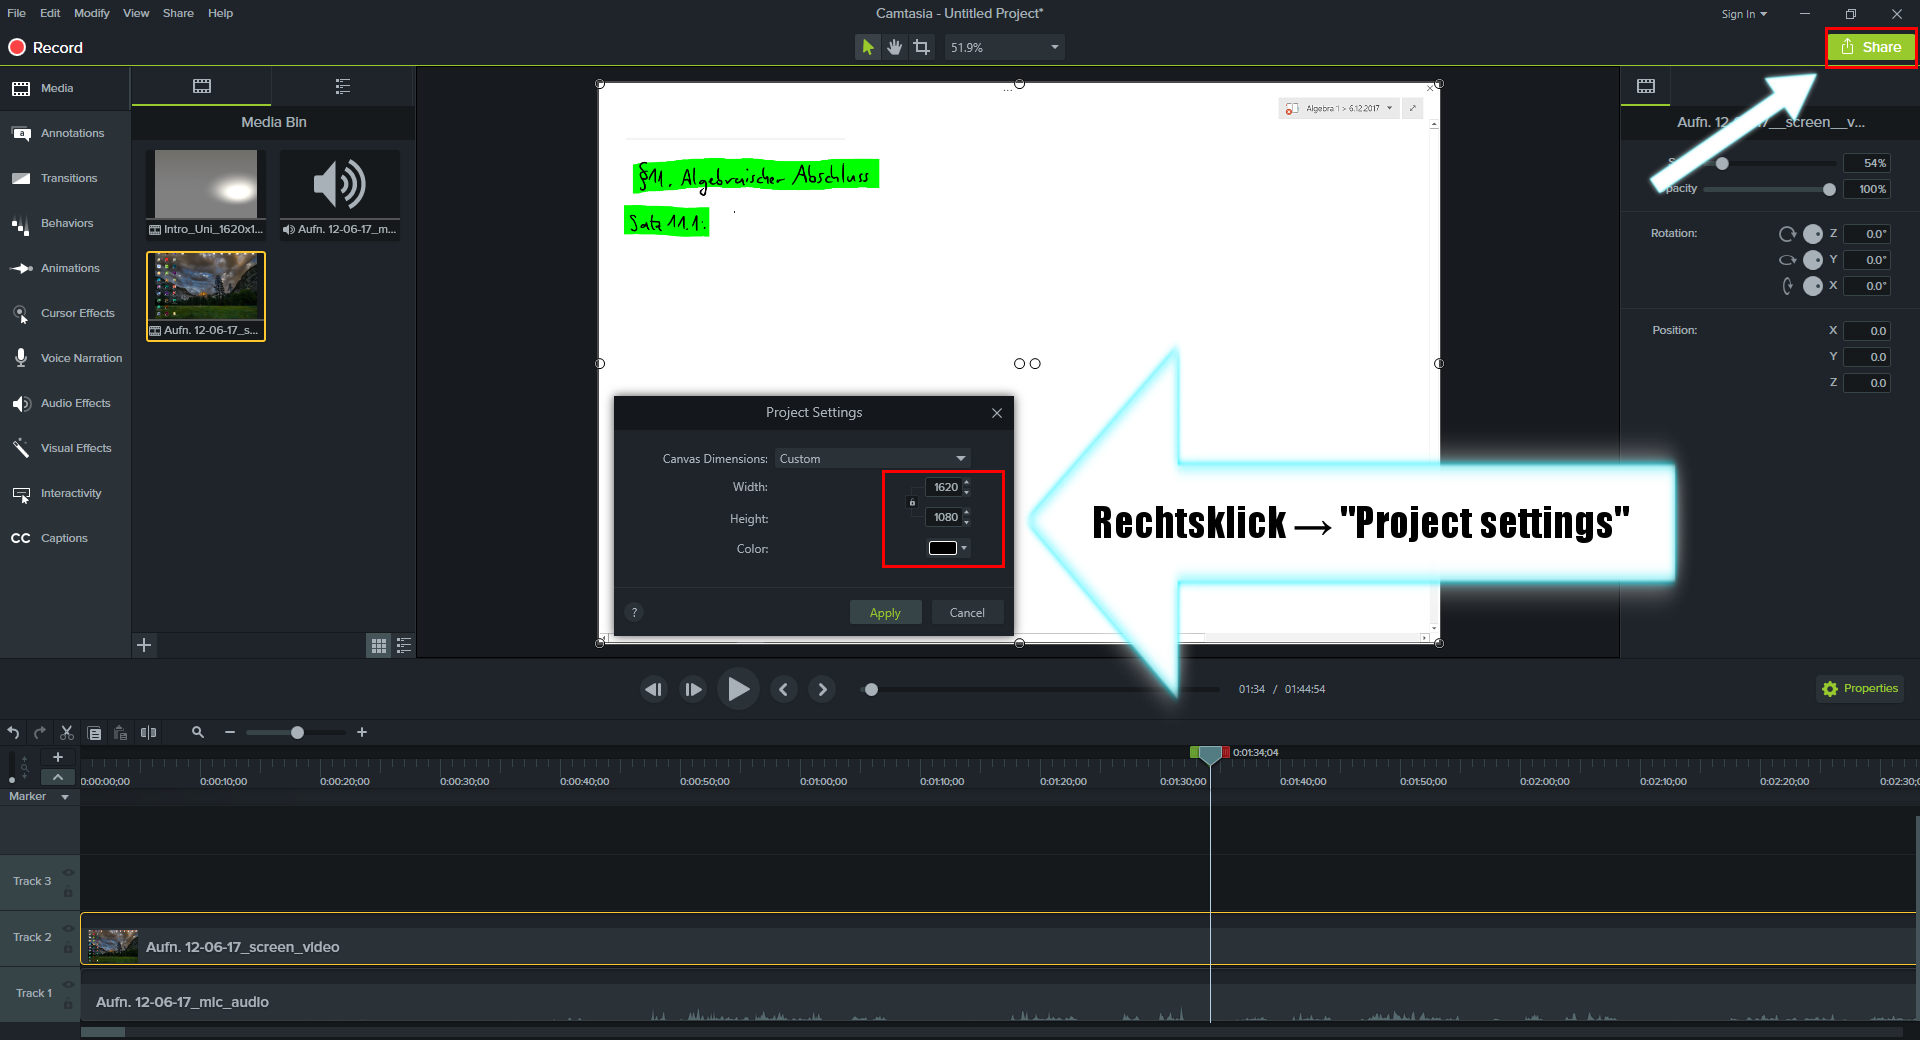
\includegraphics[width=1\textwidth]{render.png}
    \caption{Bevor das Video über ''Share'' rausgerechnet werden kann, wird die Auflösung des Projekts angepasst}
    \label{fig:render}
\end{figure}
\\
Alle Angaben bis auf die der ''Embedded Size'', welche auf 720x1080 angepasst werden sollte, können bei ihren Voreinstellungen belassen werden und die Fertigstellung des Videos kann eingeleitet werden. Das entstandene Video wird nun auf die MaMpf-Plattform hochgeladen und den Studenten zugänglich gemacht. 

\chapter{Möglichkeiten und Mehrwert digitaler und interaktiver Lerninhalte am Beispiel der Plattform MaMpf}
\section{Vorlesungsbegleitende Quizze [KeKs]}
Zusätzlich zu den Möglichkeit der Vorlesungsaufzeichnung und der digitalen Bereitsstellung selbiger, ermöglicht der Fokus auf moderne und interaktive Lernvermittlungsmethoden weitere ergänzenswerte Chancen.\\
Als Beispiel soll hier die zu MaMpf zugehörige Plattform KeKs genannt werden, bei der es sich um eine umfangreiche Datenbank handelt, in der Fragen zu klassischen Mathematikvorlesungen  der  ersten  Semester  abgespeichert sind. Durch die reichhaltige Möglichkeit, das eigene Wissen um die gerade erlernten Inhalte durch die Beantwortung von Quizfragen zu testen und zu vertiefen, erhält der Lernende einen nützlichen und hilfreichen Lernbonus.\\
\begin{figure}[h]
    \centering
    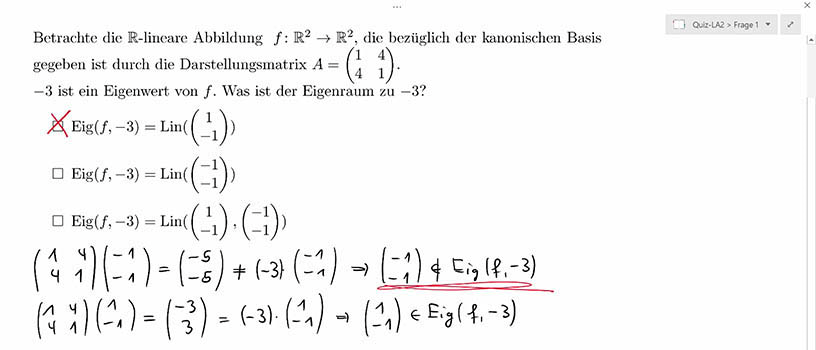
\includegraphics[width=1\textwidth]{quiz_erklaerung.png}
    \caption{Ein Beispiel für den Einsatz von KeKs inklusive Lösungsfeedback}
    \label{fig:quiz_erklaerung}
\end{figure}
\\
Im Zuge der Weiterentwicklung digitaler Lerninhalte und des Bereiches ''Video'', wäre es denkbar, die Plattform in Zukunft durch die Ergänzung um weitere, von Vorlesungen entkoppelte Videoinhalte zu ergänzen. Diese könnten in erklärender Funktion an die Quizergebnisse angeheftet werden, um einen weiteren Lernfortschritt zu erzielen. 
\section{Weitere Anwendungsgebiete [SeSam und ErDBeere]}
Abseits von den bereits erwähnten Quizzen, existieren weitere Wege, bereits hochgeladene Lernvideos durch die einbettende E-Learning Plattform sinnreich zu ergänzen. So zum Beispiel die in Kapitel 2.3 erwähnte Möglichkeit, bereits im Schnittprozess einen interaktiven Link an eine bestimmte Position des Videos platzieren, um beispielsweise ein PDF-Dokument oder eine andere hochgeladene Vorlesung zu verlinken, wodurch zusätzliche Übungsbeispiele aufgezeigt oder detailiertere Erklärungen präsentiert werden können.\\
Als weitere, abschließende Beispiele für die Anwendungsfelder digitaler Lehrvermittlung anhand von MaMpf, seien noch die Datenbanken ErDBeere (Datenbank mathematischer Beispiele und Objekte mit Suchfunktion) und SeSam (Sammlung von Beispielen zur Anwendung  klassischer Algorithmen und Methoden) erwähnt. Speziell für Letztere könnte durch die vielfältige Videoproduktion mit KaViaR zukünftig ein erheblicher Mehrwert erzielt werden und anwendungsbasierte Zusatzaufgaben durch kurze Erklärvideos ergänzt werden.
\section{HSE PLACE-Projekt}
Im Zuge des von der HSE (Heidelberg School of Education) geförderten (?) Projektes PLACE wurde zudem eine Reihe an vorlesungsbegleitenden Lehrvideos in Auftrag gegeben. Diese Lehrvideos mit einer durchschnittlichen Länge von 15 Minuten reihen sich in die bisherigen Videos von SeSAM ein und dienen dem Zweck, konkrete Methoden, Algorithmen oder Begriffe aus der Vorlesung "Lineare Algebra 1"anhand von Beispielen zu erläutern (z.B. Invertierung von Matrizen oder Äquivalenzrelationen). Für diese Videos wurde ein gesondertes Intro mit Camtasia erstellt und ähnliche Schnittprozesse durchgeführt wie im Fall der Vorlesungsvideos. Da die Videolänge jedoch hier um ein Vielfaches geringer ist, ist es nicht zwingend notwendig, die aufgenommene Videodatei mit dem MediaCoder zu komprimieren sondern kann theoretisch direkt mit Camtasia verarbeitet werden. 



\end{document}
